%%
%% This is file `mcmthesis-demo.tex',
%% generated with the docstrip utility.
%%
%% The original source files were:
%%
%% mcmthesis.dtx  (with options: `demo')
%%
%% -----------------------------------
%%
%% This is a generated file.
%%
%% Copyright (C)
%%       2010 -- 2015 by Zhaoli Wang
%%       2014 -- 2019 by Liam Huang
%%       2019 -- present by latexstudio.net
%%
%% This work may be distributed and/or modified under the
%% conditions of the LaTeX Project Public License, either version 1.3
%% of this license or (at your option) any later version.
%% The latest version of this license is in
%%   http://www.latex-project.org/lppl.txt
%% and version 1.3 or later is part of all distributions of LaTeX
%% version 2005/12/01 or later.
%%
%% This work has the LPPL maintenance status `maintained'.
%%
%% The Current Maintainer of this work is Liam Huang.
%%
%%
%% This is file `mcmthesis-demo.tex',
%% generated with the docstrip utility.
%%
%% The original source files were:
%%
%% mcmthesis.dtx  (with options: `demo')
%%
%% -----------------------------------
%%
%% This is a generated file.
%%
%% Copyright (C)
%%       2010 -- 2015 by Zhaoli Wang
%%       2014 -- 2019 by Liam Huang
%%       2019 -- present by latexstudio.net
%%
%% This work may be distributed and/or modified under the
%% conditions of the LaTeX Project Public License, either version 1.3
%% of this license or (at your option) any later version.
%% The latest version of this license is in
%%   http://www.latex-project.org/lppl.txt
%% and version 1.3 or later is part of all distributions of LaTeX
%% version 2005/12/01 or later.
%%
%% This work has the LPPL maintenance status `maintained'.
%%
%% The Current Maintainer of this work is Liam Huang.
%%
\documentclass{mcmthesis}
\mcmsetup{CTeX = false,    % 使用 CTeX 套装时,设置为 true
          tcn = {114514}, problem = \textcolor{red}{C},
          sheet = true, titleinsheet = true, keywordsinsheet = true,
          titlepage = false, abstract = false}
        
\usepackage{newtxtext}     % \usepackage{palatino}
\usepackage[backend=bibtex]{biblatex}   % for RStudio Complie
\usepackage{tabularray}
\usepackage{caption} % for table caption
\usepackage{tocloft}
\usepackage{hyperref}
\setlength{\cftbeforesecskip}{6pt}
\renewcommand{\contentsname}{\hspace*{\fill}\Large\bfseries Contents \hspace*{\fill}}

\title{Changing Tides: Momentun Swings in Tennis}
% \author{\small \href{http://www.latexstudio.net/}
%   {
\includegraphics[width=7cm]{mcmthesis-logo}}}
\date{\today}

\begin{document}

\begin{abstract}

  Situations change rapidly in tennis, and the incredible swings are often attributed to \textbf{momentum}. 
  We analyze momentum through Wimbledon 2023 men’s matches data.\par
  For Task 1, we develop a \textbf{Leverage Quantitative Momentum Capture Model}. Firstly,
  we consider the effect of short-term motivation and confidence boosting on serve percentage,
  and utilize the \textbf{Monte Carlo} algorithm to compute the winning probability(match/set/game)
  at each point. Then we define \textbf{Leverage} as how much winning or losing a ball changes the
  winning probability and the momentum as \textbf{exponential moving average} of leverage. Finally,
  the Wimbledon final match flow is visualized and the results are shown.\par
  For Task 2, we use a statistical test to verify that "momentum" does play role in the match.
  Through the \textbf{run test}, we found that at a $90\%$ confidence level, the proportion of non-random
  game scores in the given dataset accounts for $45.11\%$ of the total, which indicates the swings in
  the game are not random. Furthermore, through the contingency table independence test, we
  determine, at a $90\%$confidence level, that swings in play and runs of success by one player are
  correlated to the momentum.\par
  For Task 3, we establish the \textbf{Grid-Search Random Forest Swing Predictor Model} to forecast short-term 
  swings in momentum.We select 43 indicators as inputs for the model to predict
  \textbf{momentum transition scenarios} (no transition of advantage, the advantage tilting towards
  oneself, the advantage transitioning to the opponent) in the next s points. The model achieved a
  $94\%$ successful classification rate on the training set, demonstrating good classification performance. 
  Utilizing GSRF, we can also identify that the factor most related to match fluctuations
  is the \textbf{opponent’s total score}.\par
  It is necessary to consider he top 15 factors in the GSRF model in terms of feature importance,
  so the four factors of dimensionality reduction into \textbf{Expenditure, Expenditure, Running
  Distance, and Game Situation Factor} are utilized by \textbf{factor analysis}. We suggest players
  focus on improving physical fitness, enhancing mental resilience, and paying special attention
  to break and net point scoring techniques.\par
  For Task 4 , by modifying the Monte Carlo simulation winning rule to \textbf{three sets to two
  wins1}, we apply the model in the 2023 \textbf{Wimbledon women’s singles final}, which verifies that
  the model is generalizable. It is worth noting that the most related factor of swing in women’s
  tennis is different from that in men’s singles, it is precise \textbf{the total running distance}, which
  may be be related to the physical strength difference between men and women.\par
  We conduct \textbf{sensitivity analysis} on the parameters of the short-term motivation effect in
  the Leverage Quantitative Momentum Capture Model and the parameters in the GSRF Swing
  Predictor Model, which are low in sensitivity and have high robustness.\par
  Finally, a one-page memo with suggestions to tennis coaches is also produced to help coaches
  instruct players to control the pace of play.
  
\begin{keywords}
  Monte Carlo Simulation, Runs Test, GSRF, Factor Analysis
\end{keywords}

\end{abstract}

\maketitle

%% Generate the Table of Contents, if it's needed.
% \renewcommand{\contentsname}{\centering Contents}
\tableofcontents        % 若不想要目录, 注释掉该句
\thispagestyle{empty}

\newpage

\section{Introduction}

\subsection{Background}

Tennis matches are exciting and ever-changing. Players who seem to be dominating experience incredible swings 
from time to time. For example, a player may be in control of the
match with a series of points, but at one rally, the opponent suddenly breaks and the situation is
reversed. We often attribute this dramatic turn of events to "momentum".\par
"Momentum" heightens emotional intensity in the match, creating unpredictability and
anticipation, making each moment charged and intense.

\begin{figure}[h] 
  \centering
  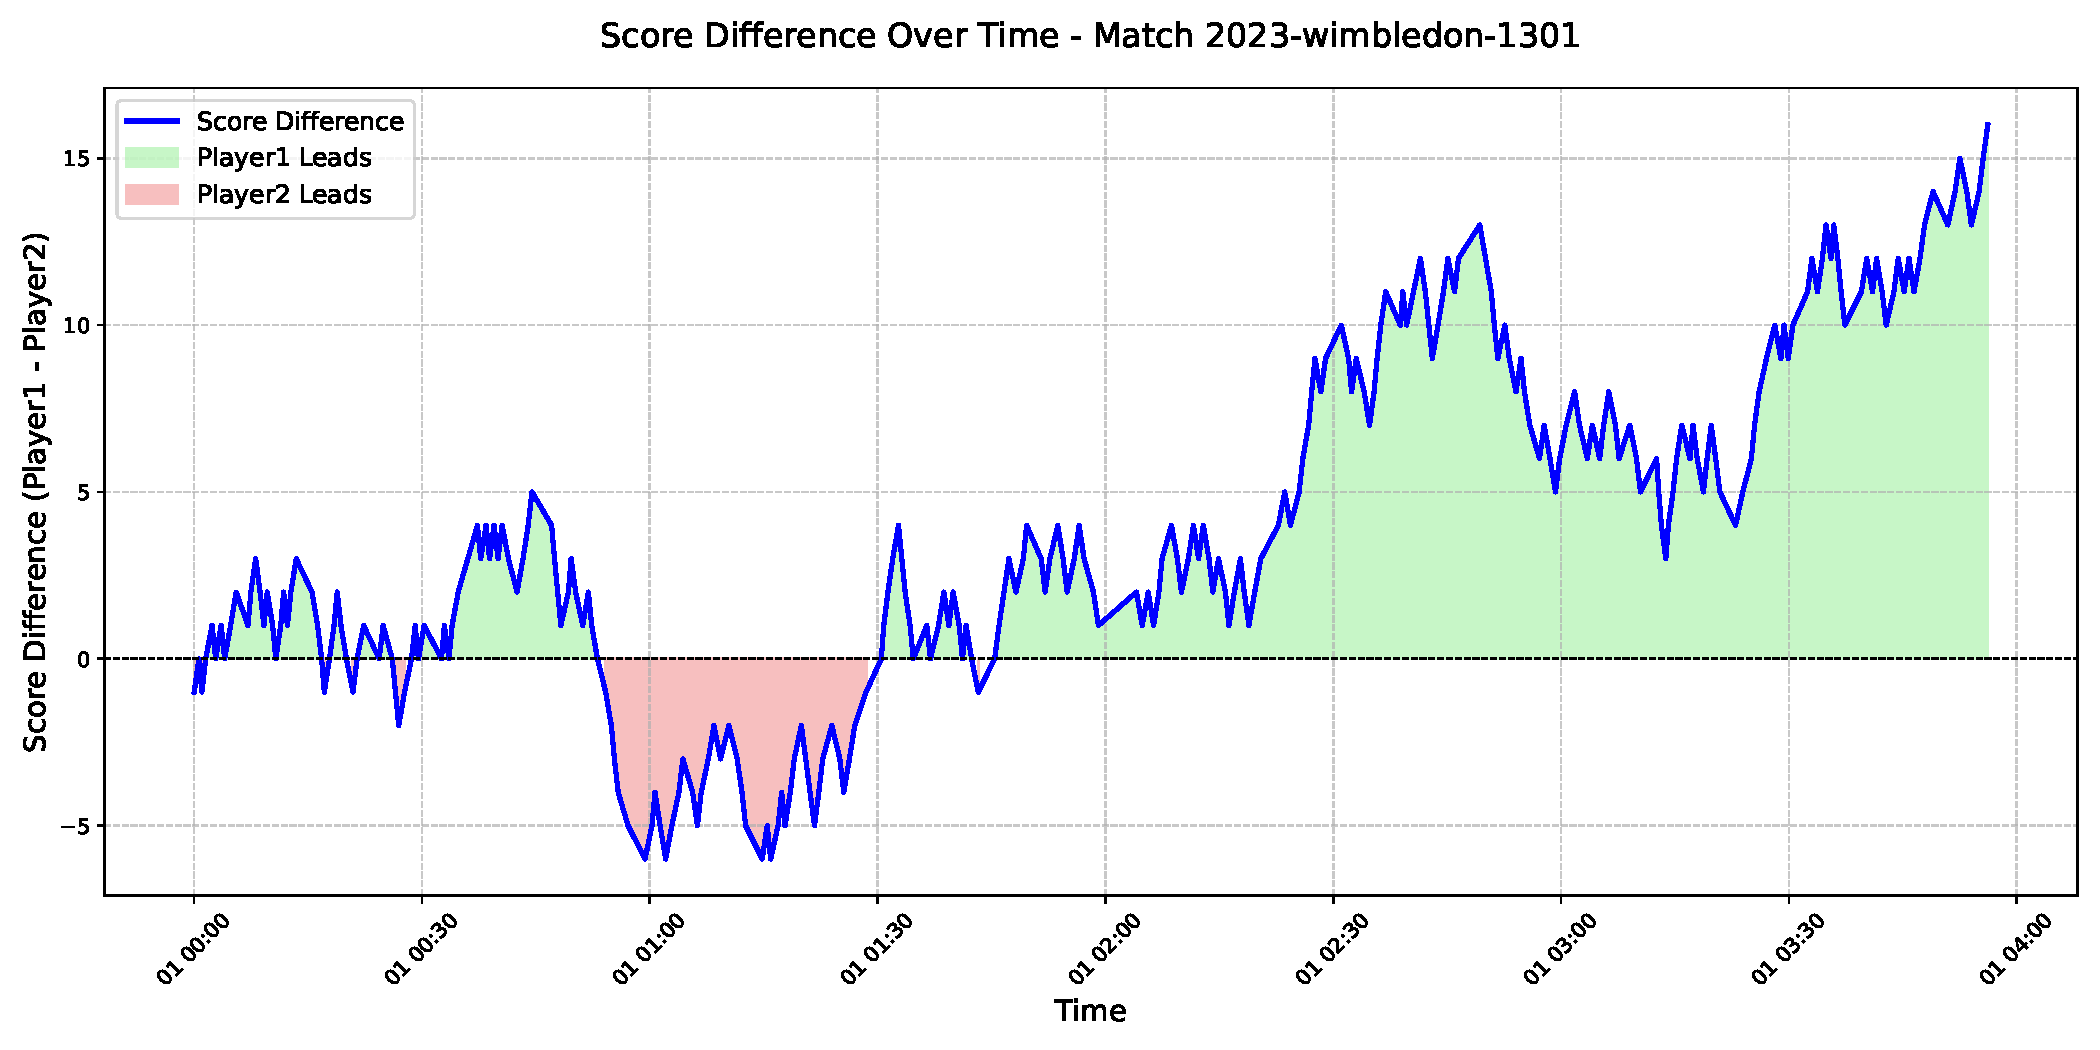
\includegraphics[width=12cm]{Score_Difference_Over_Time.pdf}
  \caption{The fast-changing, heart-stopping swings of a tennis match.} \label{fig1}
  \end{figure}

  \subsection{Restatement and Analysis of the Problem}

  We need to complete the following tasks based on the data given in the question and
  additional data from ourselves:
  \begin{itemize}
    \item \textbf{Task 1: Build a model to capture the flow of play as points occur.} 
    The model is required to be able to qualitatively and quantitatively describe 
    performance of players at a given time and provide a visualization. In particular,
    the model should take the higher probability of the server winning into account.
    \item \textbf{Task 2: Assess whether swings in play and runs of success by one player during a match 
    are random.}
    \item \textbf{Task 3: Look for indicators that identify the point in time when the game situation is reversed.}
    \begin{itemize}
      \item Develop a model to predict swings in a match. Find the indicator with the highest correlation.
      \item Based on momentum swings in past games, we need to give players advice on how to deal with other opponents.
    \end{itemize}
    \item \textbf{Task 4: Evaluate the generalisability of the model we have developed to other competitions.}
    \item \textbf{Task 5: Write a memo summarising the results and giving targeted advice to coaches and players.}
  \end{itemize}

After some analysis, we found that there is a close relationship between the tasks: In Task
1 and Task 2, we need to build a model describing the situation of the game (i.e. the relative
performance of two players) and explore the relationship between "momentum" and changes in
the game situation, respectively. The results of these two tasks are the basis of task 3. In task
3, we need to further build a model that can predict the situation fluctuations in the competition
and find out the key factors that affect the competition. We also need to start to consider the
applicability of our model. Can it provide competition suggestions for players to achieve better
results? The fourth task is to consider the extensibility of our model. Are we still valuable in
other competitions? Finally, in the memo, we need to focus on our model and its value.

In summary, we should effectively build a model that can predict the fluctuations of the
competition situation, provide practical advice to players and coaches, and be extensible across
different competitions.
\subsection{Overview of Our Work}

On the basis of the above analysis, we have carried out our work. Our working framework
is shown in Figure 2.

\begin{figure}[h] 
  \centering
  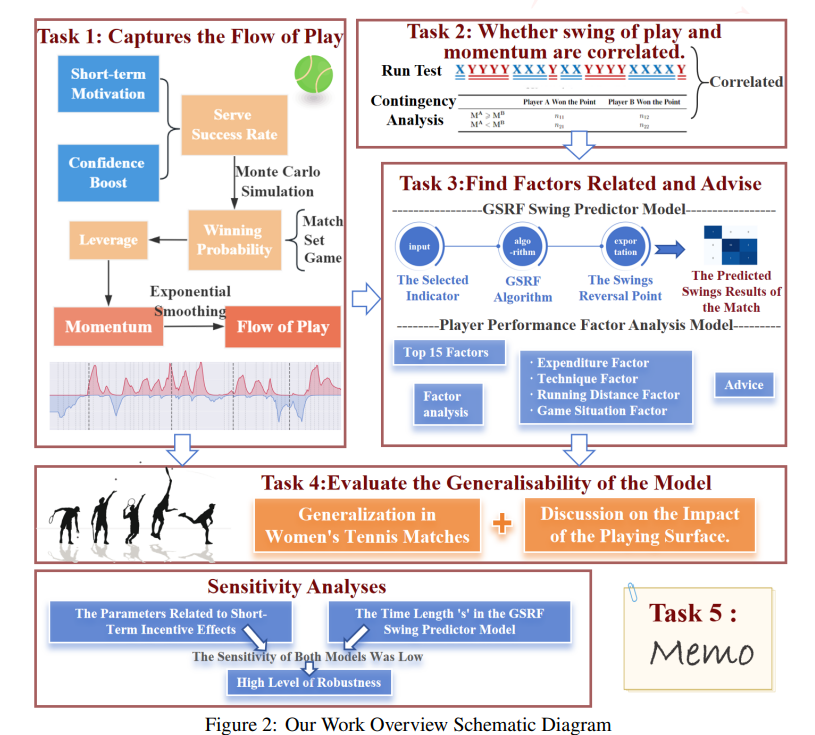
\includegraphics[width=12cm]{WorkOverview.png}
  \caption{How To Draw?} \label{fig2}
  \end{figure}
  The detailed modeling process and model details are presented in the following article.

\section{Assumptions and Justification}
To simplify the problem and make it convenient for us to simulate real-life conditions, we
make the following basic assumptions, each of which is properly justified.
\begin{itemize}
  \item \textbf{When a player wins a point, he experiences a short-term "motivational" effect
  that increases the probability of winning the next point.} The motivation effect can
lead to increased self-confidence on a psychological level as well as increased physical
conditioning on a physiological level.
  \item \textbf{Lifting effects are cumulative.} A string of successes may have a positive psychological
  and emotional effect on a player, so that a player winning more points in a row will result
  in a greater probability of winning the next point on serve.
\end{itemize}
\section{List of Notation}

\begin{table}[h]
  \centering
  \begin{tblr}{
    colspec = {X[c]X[c]}, % 自动调整列宽
    cells = {c},
    hline{1-2,9} = {-}{},
  }
  \textbf{Symbol} & \textbf{Meaning} \\
  $p,q$      & Probability of Winning       \\
  $m_i$      & Increase in the Rate of Serve points       \\
  $T_{AB}$   & The Cumulative Total Score       \\
  $L_i$      & Leverage of the $i$th Point       \\
  $G$        & The leverage Gained       \\
  $M$        & Momentum       \\
  $\lambda$  & Tuning Parameter       
  \end{tblr}
  \caption*{Noted: Symbols not specified in the table should be referred to their first occurrence.} 
\end{table}

\section{Data Pre-processing}
\begin{itemize}
  \item \textbf{Outlier Handling}
  
  No clear outliers were observed in the data. However, in a match between Frances Tiafoe
  and Grigor Dimitrov during the third round, a notable occurrence occurred with a 24-hour
  time gap between two points at a set score of 2:0, as shown in Table 1.
% \usepackage{color}
% \usepackage{tabularray}
\definecolor{Celadon}{rgb}{0.784,0.898,0.701}
\definecolor{Mercury}{rgb}{0.905,0.901,0.901}
\begin{table}[h]
\centering
\caption{ Suspected Outliers}
\begin{tblr}{
  row{1} = {Celadon,c},
  row{2} = {c},
  row{3} = {Mercury,c},
  row{4} = {c},
  row{5} = {Mercury,c},
  cell{3}{4} = {fg=red},
  cell{4}{4} = {fg=red},
}
\textbf{match\_id}  & \textbf{playerA} & \textbf{playerB} & \textbf{elapsed\_time} \\
2023-wimbledon-1303 & Frances Tiafoe   & Grigor Dimitrov  & 0:53:55                \\
2023-wimbledon-1303 & Frances Tiafoe   & Grigor Dimitrov  & 0:54:22                \\
2023-wimbledon-1303 & Frances Tiafoe   & Grigor Dimitrov  & 24:56:34               \\
2023-wimbledon-1303 & Frances Tiafoe   & Grigor Dimitrov  & 24:57:00                                
\end{tblr}
\end{table}

Upon consulting relevant information, we found the following explanation:\\
". . . . . . Saturday’s game was suspended due to inclement weather, so it was postponed to
a day later to continue on Sunday.. . . . . . "\\
Therefore, the data is correct.
  \item \textbf{Missing Value Handling}
  
  Missing Value Handling In the dataset given in the question,the quantities $serve_{width}$,
  $serve_{depth}$,and $return_{depth}$ have missing values,for which we use the \textbf{nearest-neighbour} 
  filling method to fill them. 
  \item \textbf{Tag Encoding of String Type Data} 
  
  There are many categorical variables in the data given in the title, presented as strings. In order to make it 
  easier for the model to receive this type of data,we preprocess this type of data by 
  means of label coding, using virtual coding for the last three columns of $serve_{width}$,
  $serve_{depth}$,and $return_{depth}$ in the data of the tennis match.
\end{itemize}

\section{Task1: Captures the Flow of Play}
\subsection{Soecifying Conceptual Significance}
Since a relatively large number of concepts are introduced in our model, we first identify
and clarify the meaning of the introduced concepts here.
\begin{itemize}
  \item \textbf{Short-term Motivation} refers to a brief period of above-average performance by a player
  following a motivating event.
  \item \textbf{Confidence Boost} is when a player, drawing upon their self-awareness developed through
  multiple games in their professional career and an assessment of the current situation,
  generates positive expectations regarding the outcome of the match.
  \item \textbf{Serve Success Rate} is probability of scoring in a service game.
  \item \textbf{Winning Probability} is the likelihood of the player winning the game/set/match.
  \item \textbf{Leverage} measures how a ball’s outcome impacts the margin of victory.
  \item \textbf{Momentum} aims to describe which player is in control at any given point in the
  match—based on who is currently winning more points and who is prevailing in crucial
  (high-leverage) moments. It is defined as a player’s exponentially weighted leverage
  average.\par
  At each point in the match, both competing players will have their own momentum values.
  \item We define the fluctuations in momentum as the \textbf{Flow of Play.}
\end{itemize}
The relationship between the above concepts, i.e., the framework of the model, 
is shown schematically below, and in the following we show the model building process in full.
\subsection{Leverage Quantitative Momentum Capture Model}
\subsubsection{Impact of Short-term Motivation and Confidence Boost on Serve Success Rate}
\textbf{Short-term Motivation} refers to a brief period of above-average performance by a player
following a motivating event (e.g., a breaking serve) during a match, a phenomenon known
in sports as "hot hands". We developed a probabilistic model that quantifies Short-term
Motivation as an increase in serve success rate.\par
The following two assumptions are necessary:
\begin{itemize}
  \item When a player wins a point, he experiences a short-term "motivational" effect that increases
  the probability of winning the next point.
  \item Lifting effects are cumulative. A string of successes may have a positive psychological
  and emotional effect on a player, so that a player winning more points in a row will result
  in a greater probability of winning the next point on serve.
\end{itemize}
Here $i$ denotes the number of consecutive points scored by a player $A$ or his opponent $B$;
and $m_i$ denotes the increase in the rate of serving points on a player’s next serve after winning
$i$points consecutively due to the short-term motivation gained. Then, the probability of winning
the next serve under short-term motivation $p_s$ versus $q_s$ is calculated by \eqref{eq01}.
\begin{equation}
  \begin{split}
    p_s &= p_f(1+m_i^A);\\
    q_s &= q_f(1+m_i^B),
  \end{split}
  \label{eq01}
\end{equation}
where $p_f$ and $q_f$ are the scoring probabilities before player $A$ and player $B$ are motivated,
respectively.\par
The short-term motivation that a player receives for scoring a game $n$ times in a row is
referred to as $n$-order short-term motivation. Using the dataset given in the title, we statistically
obtained a plot of the total number of short-term motivations occurring in a match versus order,
and the results are shown in Figure \ref{fig3}. \par
\begin{figure}[h]
  \centering
  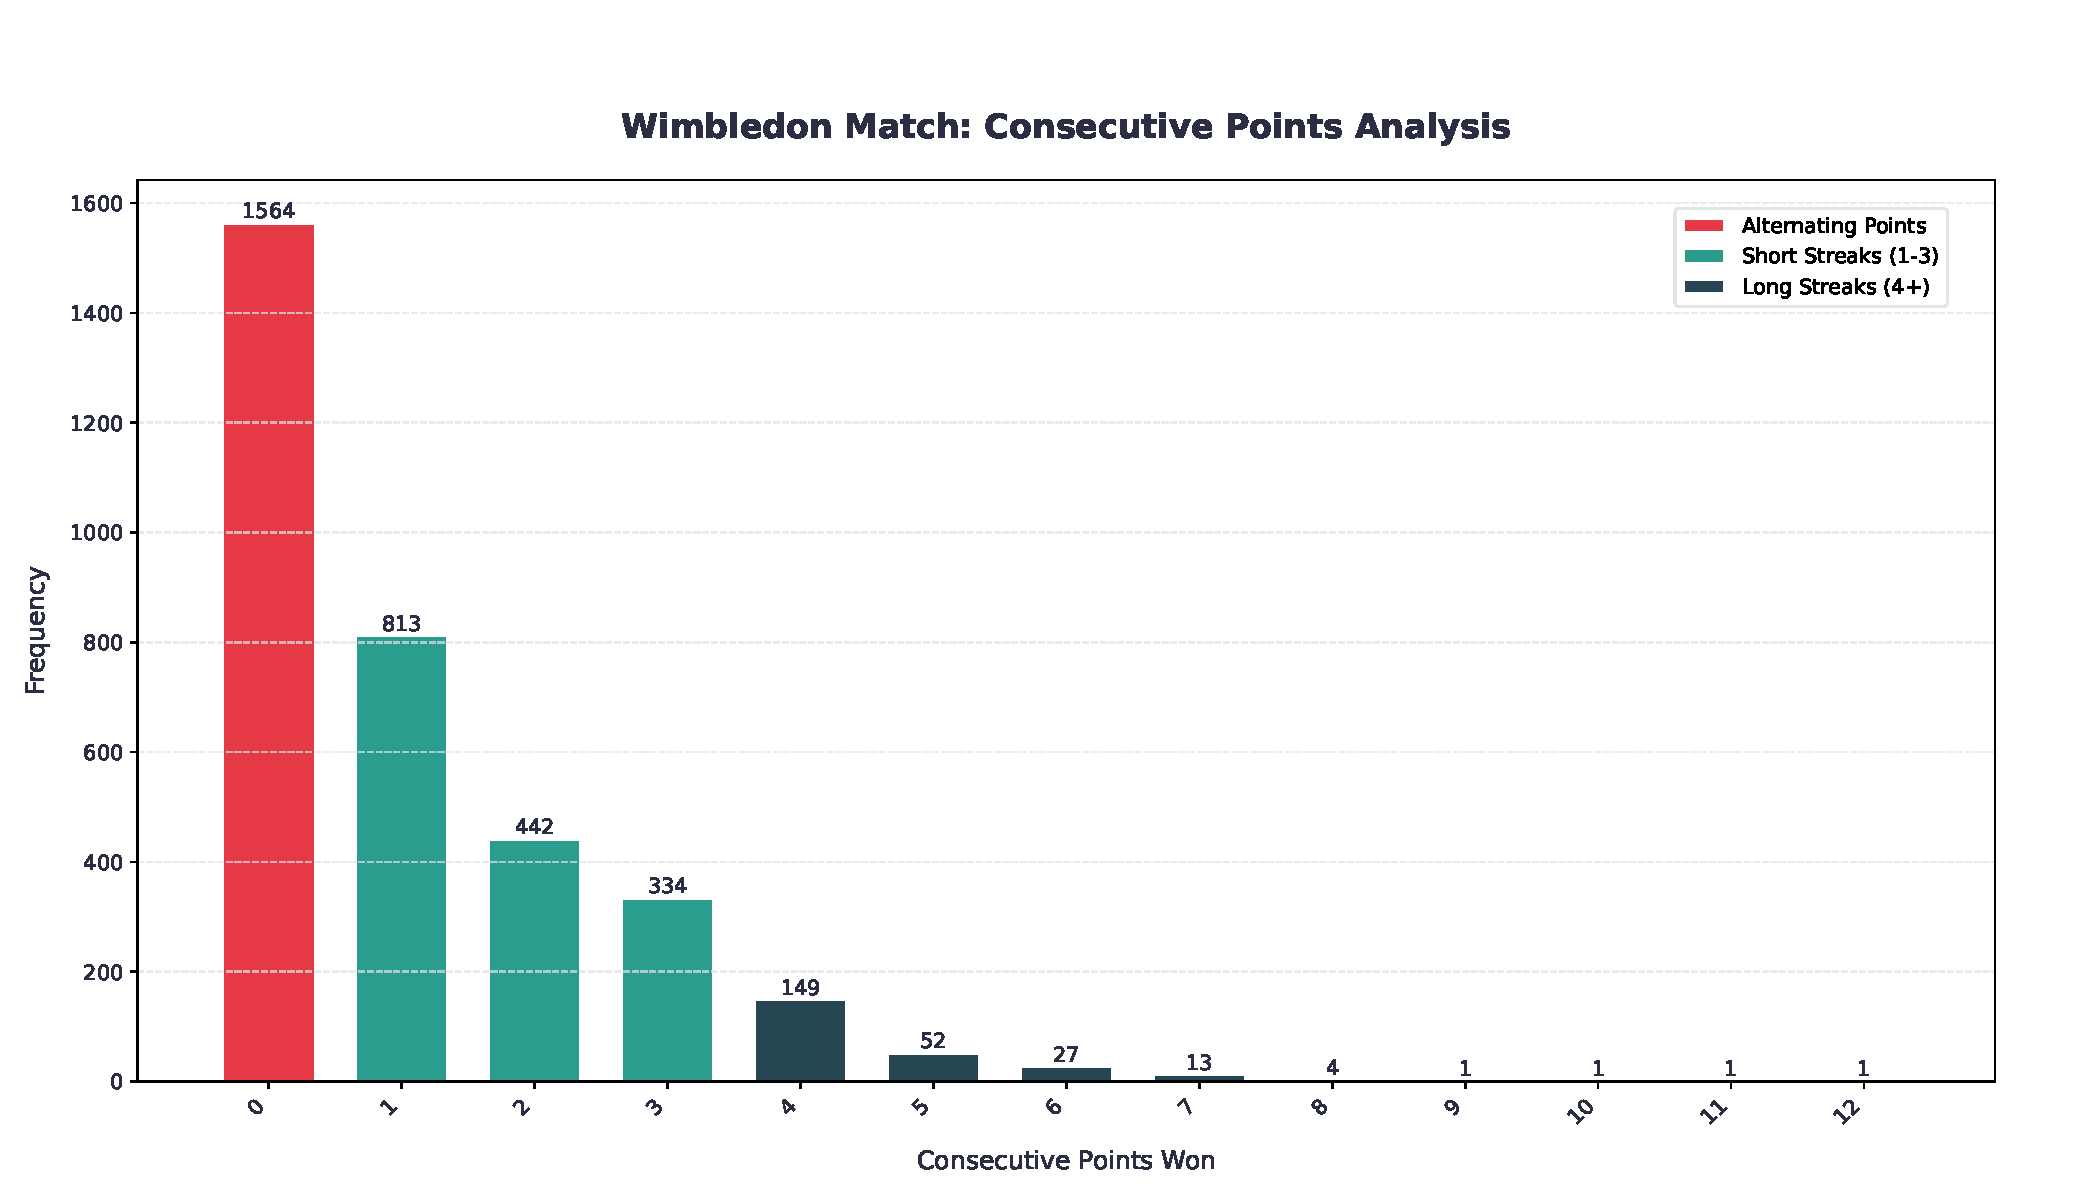
\includegraphics[width=12cm]{continue_winning.pdf}
  \caption{The number of short-term motivations of different orders in a match.} \label{fig4}
  \label{fig3}
\end{figure}
It is clear to see that short-term motivations of order four
and above rarely occur in the dataset used in this study. Therefore, only short-term motivations
of order three and below are considered in this paper.\par
Short-termmotivation focuses on short-termstatus enhancement during matches and ignores
sources of motivation on a longer time scale in the player’s lifetime, so we continue to introduce
a \textbf{confidence-boosting factor}.\par
A new tuning parameter $\lambda$ is introduced, which represents the effect of the confidence
boosting factor on the success rate of the next serve, the probabilities after the effect are
expressed as $p_s$ and $q_s$ – see equation \eqref{eq02}
\begin{equation}
  \begin{split}
    p_c = \frac{T_{AB}}{\lambda} p_t + \left(1 - \frac{T_{AB}}{\lambda}\right) p_0;\\
  q_c = \frac{T_{AB}}{\lambda} q_t + \left(1 - \frac{T_{AB}}{\lambda}\right) q_0,
  \end{split}
  \label{eq02}
\end{equation}
where $T_{AB}$ denotes the cumulative total score of the opposing players since the start of the
match, and $p_t$ and $q_t$ denote the probability of scoring for player $A$ and player $B$, respectively,
since the start of the match up to the present. $p_0$ and $q_0$ denote the historical data on the success
rate of the opposing teams’ serves on the grass court surface prior to the current match (source:
\url{https://www.infosys.com/})\par
Eq. (2) describes the phenomenon that a player’s historical results always have the greatest
impact on player status at the start of a match, and then diminish as the match progresses - the
performance of the current match begins to influence player play more.\par
We then performed a linear interpolation of the obtained probabilities. The interpolation
coefficient is the cumulative total score of the current pair divided by the coefficient $\lambda$ (i.e.$\frac{T_{AB}}{\lambda}$).\par
The short-term motivation is fluctuating as the match progresses, while the confidence boost
takes into account the player’s self-perception established over the course of his career as well
as the current situation in the match, which is the "undertone" of the motivated state, therefore,
we use $pc$ and $qc$ in Eq. \eqref{eq02} instead of $p_f$ and $q_f$ in Eq. \eqref{eq01}, we can get the success rate of the
next serve after considering the short-term motivation and confidence improvement:
\begin{equation*}
  \begin{split}
    p = \left[ \frac{T_{AB}}{\lambda} \cdot p_c + \left( 1 - \frac{T_{AB}}{\lambda} \right) p_t \right] (1 + m_i^A);\\
    q = \left[ \frac{T_{AB}}{\lambda} \cdot q_c + \left( 1 - \frac{T_{AB}}{\lambda} \right) q_t \right] (1 + m_i^B).
  \end{split}
\end{equation*}
The above equation shows the effect of short-term motivation and confidence enhancement
on serve percentage.\par
In tennis matches, players typically have an advantage when serving. According to the
data we have collected, the serving success rate of professional players exceeds $50\%$. Based
on this understanding, \textbf{players gain confidence in serving games.} Due to this "confidence
boost," we have incorporated the player’s performance in serving games into consideration in
our model.
\subsubsection{Monte Carlo Simulation for Winning Probability}
\begin{center}
\begin{tabular}{clc}
{\bf Symbols} & {\bf Description} & \quad {\bf Unit} \\[0.25cm]
$h$ & Convection heat transfer coefficient & \quad W/(m$^2 \cdot$ K) 
\\[0.2cm]
$k$ & Thermal conductivity & \quad W/(m $\cdot$ K) \\[0.2cm]
$c_p$ & Specific heat & \quad J/(kg $\cdot$ K) \\[0.2cm]
$\rho$ & Density & \quad kg/m$^2$ \\[0.2cm]
$\delta$ & Thickness & \quad m \\[0.2cm]
$t$ & Temperature & \quad $^\circ$C, K \\[0.2cm]
$\tau$ & Time & \quad s, min, h \\[0.2cm]
$q_m$ & Mass flow & \quad kg/s \\[0.2cm]
$\Phi$ & Heat transfer power & \quad W \\[0.2cm]
$T$ & A period of time & \quad s, min, h \\[0.2cm]
$V$ & Volume & \quad m$^3$, L \\[0.2cm]
$M,\,m$ & Mass & \quad kg \\[0.2cm]
$A$ & Aera & \quad m$^2$ \\[0.2cm]
$a,\,b,\,c$ & The size of a bathtub  & \quad m$^3$
\end{tabular}
\end{center}

\noindent where we define the main parameters while specific value of those parameters will be given later.

\section{Model Overview}

In our basic model, we aim at three goals: keeping the temperature as even as possible, making it close to the initial temperature and decreasing the water consumption.

We start with the simple sub-model where hot water is added constantly.
At first we introduce convection heat transfer control equations in rectangular coordinate system. Then we define the mean temperature of bath water.

Afterwards, we introduce Newton cooling formula to determine heat transfer
capacity. After deriving the value of parameters, we get calculating results via formula deduction and simulating results via CFD.

Secondly, we present the complicated sub-model in which hot water is
added discontinuously. We define an iteration consisting of two process:
heating and standby. As for heating process, we derive control equations and boundary conditions. As for standby process, considering energy conservation law, we deduce the relationship of total heat dissipating capacity and time.

Then we determine the time and amount of added hot water. After deriving the value of parameters, we get calculating results via formula deduction and simulating results via CFD.

At last, we define two criteria to evaluate those two ways of adding hot water. Then we propose optimal strategy for the user in a bathtub.
The whole modeling process can be shown as follows.

\begin{figure}[h] 
\centering
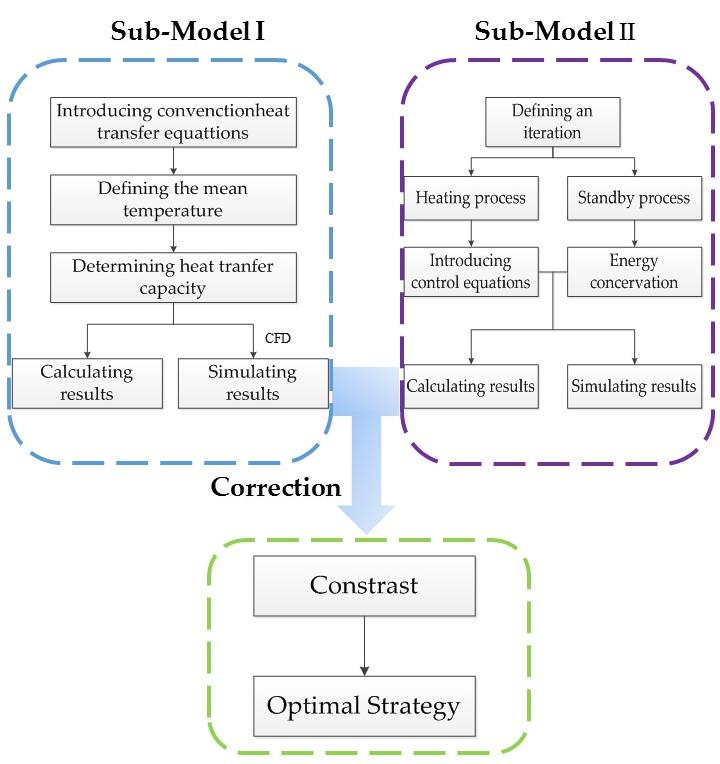
\includegraphics[width=12cm]{fig1.jpg}
\caption{Modeling process} \label{fig1}
\end{figure}

\section{Sub-model I : Adding Water Continuously}

We first establish the sub-model based on the condition that a person add water continuously to reheat the bathing water. Then we use Computational Fluid Dynamics (CFD) to simulate the change of water temperature in the bathtub. At last, we evaluate the model with the criteria which have been defined before.

\subsection{Model Establishment}

Since we try to keep the temperature of the hot water in bathtub to be even, we have to derive the amount of inflow water and the energy dissipated by the hot water into the air.

We derive the basic convection heat transfer control equations based on the former scientists’ achievement. Then, we define the mean temperature of bath water. Afterwards, we determine two types of heat transfer: the boundary heat transfer and the evaporation heat transfer. Combining thermodynamic formulas, we derive calculating results. Via Fluent software, we get simulation results.

\subsubsection{Control Equations and Boundary Conditions}

According to thermodynamics knowledge, we recall on basic convection
heat transfer control equations in rectangular coordinate system. Those
equations show the relationship of the temperature of the bathtub water in space.

We assume the hot water in the bathtub as a cube. Then we put it into a
rectangular coordinate system. The length, width, and height of it is $a,\, b$ and $c$.

\begin{figure}[h] 
\centering
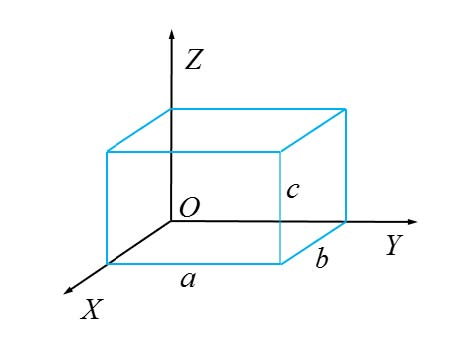
\includegraphics[width=8cm]{fig2.jpg}
\caption{Modeling process} \label{fig2}
\end{figure}

In the basis of this, we introduce the following equations \cite{5}:

\begin{itemize}
\item {\bf Continuity equation:}
\end{itemize}

\begin{equation} \label{eq1}
\frac{\partial u}{\partial x} + \frac{\partial v}{\partial y} +\frac{\partial w}{\partial z} =0
\end{equation}

\noindent where the first component is the change of fluid mass along the $X$-ray. The second component is the change of fluid mass along the $Y$-ray. And the third component is the change of fluid mass along the $Z$-ray. The sum of the change in mass along those three directions is zero.

\begin{itemize}
\item {\bf Moment differential equation (N-S equations):}
\end{itemize}

\begin{equation} \label{eq2}
\left\{
\begin{array}{l} \!\!
\rho \Big(u \dfrac{\partial u}{\partial x} + v \dfrac{\partial u}{\partial y} + w\dfrac{\partial u}{\partial z} \Big) = -\dfrac{\partial p}{\partial x} + \eta \Big(\dfrac{\partial^2 u}{\partial x^2} + \dfrac{\partial^2 u}{\partial y^2} + \dfrac{\partial^2 u}{\partial z^2} \Big) \\[0.3cm]
\rho \Big(u \dfrac{\partial v}{\partial x} + v \dfrac{\partial v}{\partial y} + w\dfrac{\partial v}{\partial z} \Big) = -\dfrac{\partial p}{\partial y} + \eta \Big(\dfrac{\partial^2 v}{\partial x^2} + \dfrac{\partial^2 v}{\partial y^2} + \dfrac{\partial^2 v}{\partial z^2} \Big) \\[0.3cm]
\rho \Big(u \dfrac{\partial w}{\partial x} + v \dfrac{\partial w}{\partial y} + w\dfrac{\partial w}{\partial z} \Big) = -g-\dfrac{\partial p}{\partial z} + \eta \Big(\dfrac{\partial^2 w}{\partial x^2} + \dfrac{\partial^2 w}{\partial y^2} + \dfrac{\partial^2 w}{\partial z^2} \Big)  
\end{array}
\right.
\end{equation}

\begin{itemize}
\item {\bf Energy differential equation:}
\end{itemize}

\begin{equation} \label{eq3}
\rho c_p \Big( u\frac{\partial t}{\partial x} + v\frac{\partial t}{\partial y} + w\frac{\partial t}{\partial z} \Big) = \lambda \Big(\frac{\partial^2 t}{\partial x^2} + \frac{\partial^2 t}{\partial y^2} + \frac{\partial^2 t}{\partial z^2} \Big)
\end{equation}

\noindent where the left three components are convection terms while the right three components are conduction terms.

By Equation \eqref{eq3}, we have ......

......

On the right surface in Fig. \ref{fig2}, the water also transfers heat firstly with bathtub inner surfaces and then the heat comes into air. The boundary condition here is ......

\subsubsection{Definition of the Mean Temperature}

......

\subsubsection{Determination of Heat Transfer Capacity}

......

\section{Sub-model II: Adding Water Discontinuously}

In order to establish the unsteady sub-model, we recall on the working principle of air conditioners. The heating performance of air conditions consist of two processes: heating and standby. After the user set a temperature, the air conditioner will begin to heat until the expected temperature is reached. Then it will go standby. When the temperature get below the expected temperature, the air conditioner begin to work again. As it works in this circle, the temperature remains the expected one.

Inspired by this, we divide the bathtub working into two processes: adding
hot water until the expected temperature is reached, then keeping this
condition for a while unless the temperature is lower than a specific value. Iterating this circle ceaselessly will ensure the temperature kept relatively stable.

\subsection{Heating Model}

\subsubsection{Control Equations and Boundary Conditions}

\subsubsection{Determination of Inflow Time and Amount}

\subsection{Standby Model}

\subsection{Results}

\quad~ We first give the value of parameters based on others’ studies. Then we get the calculation results and simulating results via those data.

\subsubsection{Determination of Parameters}

After establishing the model, we have to determine the value of some
important parameters.

As scholar Beum Kim points out, the optimal temperature for bath is
between 41 and 45$^\circ$C [1]. Meanwhile, according to Shimodozono's study, 41$^\circ$C warm water bath is the perfect choice for individual health [2]. So it is reasonable for us to focus on $41^\circ$C $\sim 45^\circ$C. Because adding hot water continuously is a steady process, so the mean temperature of bath water is supposed to be constant. We value the temperature of inflow and outflow water with the maximum and minimum temperature respectively.

The values of all parameters needed are shown as follows:

.....

\subsubsection{Calculating Results}

Putting the above value of parameters into the equations we derived before, we can get the some data as follows:

%%普通表格
\begin{table}[h]  %h表示固定在当前位置
\centering        %设置居中
\caption{The calculating results}  %表标题
\vspace{0.15cm}
\label{tab2}                       %设置表的引用标签
\begin{tabular}{|c|c|c|}  %3个c表示3列, |可选, 表示绘制各列间的竖线
\hline                    %画横线
Variables & Values & Unit     \\ \hline  %各列间用&隔开
$A_1$     & 1.05   &   $m^2$  \\ \hline
$A_2$     & 2.24   &   $m^2$  \\ \hline
$\Phi_1$  & 189.00 &   $W$   \\ \hline
$\Phi_2$  & 43.47  &   $W$   \\ \hline
$\Phi$    & 232.47 &   $W$   \\ \hline
$q_m$     & 0.014  &   $g/s$ \\ \hline
\end{tabular}
\end{table}

From Table \ref{tab2}, ......

......

\section{Correction and Contrast of Sub-Models}

After establishing two basic sub-models, we have to correct them in consideration of evaporation heat transfer. Then we define two evaluation criteria to compare the two sub-models in order to determine the optimal bath strategy.

\subsection{Correction with Evaporation Heat Transfer}

Someone may confuse about the above results: why the mass flow in the first sub-model is so small? Why the standby time is so long? Actually, the above two sub-models are based on ideal conditions without consideration of the change of boundary conditions, the motions made by the person in bathtub and the evaporation of bath water, etc. The influence of personal motions will be discussed later. Here we introducing the evaporation of bath water to correct sub-models.

\subsection{Contrast of Two Sub-Models}

Firstly we define two evaluation criteria. Then we contrast the two submodels via these two criteria. Thus we can derive the best strategy for the person in the bathtub to adopt.

\section{Model Analysis and Sensitivity Analysis}

\subsection{The Influence of Different Bathtubs}

Definitely, the difference in shape and volume of the tub affects the
convection heat transfer. Examining the relationship between them can help
people choose optimal bathtubs.

\subsubsection{Different Volumes of Bathtubs}

In reality, a cup of water will be cooled down rapidly. However, it takes quite long time for a bucket of water to become cool. That is because their volume is different and the specific heat of water is very large. So that the decrease of temperature is not obvious if the volume of water is huge. That also explains why it takes 45 min for 320 L water to be cooled by 1$^\circ$C.

In order to examine the influence of volume, we analyze our sub-models
by conducting sensitivity Analysis to them.

We assume the initial volume to be 280 L and change it by $\pm 5$\%, $\pm 8$\%, $\pm 12$\% and $\pm 15$\%. With the aid of sub-models we established before, the variation of some parameters turns out to be as follows

%%三线表
\begin{table}[h] %h表示固定在当前位置
\centering  %设置居中
\caption{Variation of some parameters}  %表标题
\label{tab7} %设置表的引用标签
\begin{tabular}{ccccccc} %7个c表示7列, c表示每列居中对齐, 还有l和r可选
\toprule  %画顶端横线
$V$      & $A_1$   & $A_2$   & $T_2$    & $q_{m1}$ & $q_{m2}$ & $\Phi_q$ \\
\midrule  %画中间横线
-15.00\% & -5.06\% & -9.31\% & -12.67\% & -2.67\%  & -14.14\% & -5.80\% \\
-12.00\% & -4.04\% & -7.43\% & -10.09\% & -2.13\%  & -11.31\% & -4.63\% \\
-8.00\%  & -2.68\% & -4.94\% & -6.68\%  & -1.41\%  & -7.54\%  & -3.07\% \\
-8.00\%  & -2.68\% & -4.94\% & -6.68\%  & -1.41\%  & -7.54\%  & -3.07\% \\
-8.00\%  & -2.68\% & -4.94\% & -6.68\%  & -1.41\%  & -7.54\%  & -3.07\% \\
-8.00\%  & -2.68\% & -4.94\% & -6.68\%  & -1.41\%  & -7.54\%  & -3.07\% \\
-8.00\%  & -2.68\% & -4.94\% & -6.68\%  & -1.41\%  & -7.54\%  & -3.07\% \\
-8.00\%  & -2.68\% & -4.94\% & -6.68\%  & -1.41\%  & -7.54\%  & -3.07\% \\
-8.00\%  & -2.68\% & -4.94\% & -6.68\%  & -1.41\%  & -7.54\%  & -3.07\% \\
-8.00\%  & -2.68\% & -4.94\% & -6.68\%  & -1.41\%  & -7.54\%  & -3.07\% \\
-8.00\%  & -2.68\% & -4.94\% & -6.68\%  & -1.41\%  & -7.54\%  & -3.07\% \\
\bottomrule  %画底部横线
\end{tabular}
\end{table}

\section{Strength and Weakness}

\subsection{Strength}

\begin{itemize}
\item We analyze the problem based on thermodynamic formulas and laws, so that the model we established is of great validity.

\item Our model is fairly robust due to our careful corrections in consideration of real-life situations and detailed sensitivity analysis.

\item Via Fluent software, we simulate the time field of different areas throughout the bathtub. The outcome is vivid for us to understand the changing process.

\item We come up with various criteria to compare different situations, like water consumption and the time of adding hot water. Hence an overall comparison can be made according to these criteria.

\item Besides common factors, we still consider other factors, such as evaporation and radiation heat transfer. The evaporation turns out to be the main reason of heat loss, which corresponds with other scientist’s experimental outcome.
\end{itemize}

\subsection{Weakness}

\begin{itemize}
\item Having knowing the range of some parameters from others’ essays, we choose a value from them to apply in our model. Those values may not be reasonable in reality.

\item Although we investigate a lot in the influence of personal motions, they are so complicated that need to be studied further.

\item Limited to time, we do not conduct sensitivity analysis for the influence of personal surface area.
\end{itemize}

\section{Further Discussion}

In this part, we will focus on different distribution of inflow faucets. Then we discuss about the real-life application of our model.

\begin{itemize}
\item Different Distribution of Inflow Faucets

In our before discussion, we assume there being just one entrance of inflow.

From the simulating outcome, we find the temperature of bath water is hardly even. So we come up with the idea of adding more entrances.

The simulation turns out to be as follows

\begin{figure}[h] 
\centering
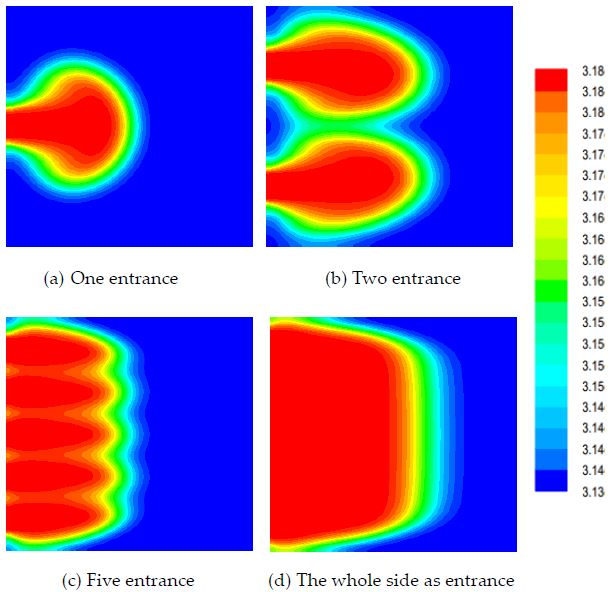
\includegraphics[width=12cm]{fig24.jpg}
\caption{The simulation results of different ways of arranging entrances} \label{fig24}
\end{figure}

From the above figure, the more the entrances are, the evener the temperature will be. Recalling on the before simulation outcome, when there is only one entrance for inflow, the temperature of corners is quietly lower than the middle area.

In conclusion, if we design more entrances, it will be easier to realize the goal to keep temperature even throughout the bathtub.

\item Model Application

Our before discussion is based on ideal assumptions. In reality, we have to make some corrections and improvement.

\begin{itemize}
\item[1)] Adding hot water continually with the mass flow of 0.16 kg/s. This way can ensure even mean temperature throughout the bathtub and waste less water.

\item[2)] The manufacturers can design an intelligent control system to monitor the temperature so that users can get more enjoyable bath experience.

\item[3)] We recommend users to add bubble additives to slow down the water being cooler and help cleanse. The additives with lower thermal conductivity are optimal.

\item[4)] The study method of our establishing model can be applied in other area relative to convection heat transfer, such as air conditioners.
\end{itemize}
\end{itemize}

\begin{thebibliography}{99}
\addcontentsline{toc}{section}{Reference}

\bibitem{1} Gi-Beum Kim. Change of the Warm Water Temperature for the Development of Smart Healthecare Bathing System. Hwahak konghak. 2006, 44(3): 270-276.
\bibitem{2} \url{https://en.wikipedia.org/wiki/Convective_heat_transfer#Newton.27s_law_of_cooling}
\bibitem{3} \url{https://en.wikipedia.org/wiki/Navier\%E2\%80\%93Stokes_equations}
\bibitem{4} \url{https://en.wikipedia.org/wiki/Computational_fluid_dynamics}
\bibitem{5} Holman J P. Heat Transfer (9th ed.), New York: McGraw-Hill, 2002. 
\bibitem{6} Liu Weiguo, Chen Zhaoping, ZhangYin. Matlab program design and application. Beijing: Higher education press, 2002. (In Chinese)

\end{thebibliography}

\newpage

\begin{letter}{Enjoy Your Bath Time!}

From simulation results of real-life situations, we find it takes a period of time for the inflow hot water to spread throughout the bathtub. During this process, the bath water continues transferring heat into air, bathtub and the person in bathtub. The difference between heat transfer capacity makes the temperature of various areas to be different. So that it is difficult to get an evenly maintained temperature throughout the bath water.

In order to enjoy a comfortable bath with even temperature of bath water and without wasting too much water, we propose the following suggestions.

\begin{itemize}
\item Adding hot water consistently
\item Using smaller bathtub if possible
\item Decreasing motions during bath
\item Using bubble bath additives
\item Arranging more faucets of inflow
\end{itemize}

\vspace{\parskip}

Sincerely yours,

Your friends

\end{letter}

\newpage

\begin{appendices}

\section{First appendix}

In addition, your report must include a letter to the Chief Financial Officer (CFO) of the Goodgrant Foundation, Mr. Alpha Chiang, that describes the optimal investment strategy, your modeling approach and major results, and a brief discussion of your proposed concept of a return-on-investment (ROI). This letter should be no more than two pages in length.

Here are simulation programmes we used in our model as follow.\\

\textbf{\textcolor[rgb]{0.98,0.00,0.00}{Input matlab source:}}
\lstinputlisting[language=Matlab]{./code/mcmthesis-matlab1.m}

\section{Second appendix}

some more text \textcolor[rgb]{0.98,0.00,0.00}{\textbf{Input C++ source:}}
\lstinputlisting[language=C++]{./code/mcmthesis-sudoku.cpp}

\end{appendices}

\newpage
\newcounter{lastpage}
\setcounter{lastpage}{\value{page}}
\thispagestyle{empty} 

\section*{Report on Use of AI}

\begin{enumerate}
\item OpenAI ChatGPT (Nov 5, 2023 version, ChatGPT-4,) 
\begin{description}
\item[Query1:] <insert the exact wording you input into the AI tool> 
\item[Output:] <insert the complete output from the AI tool>
\end{description}
\item OpenAI Ernie (Nov 5, 2023 version, Ernie 4.0) 
\begin{description}
\item[Query1:] <insert the exact wording of any subsequent input into the AI tool> 
\item[Output:] <insert the complete output from the second query>
\end{description}
\item Github CoPilot (Feb 3, 2024 version) 
\begin{description}
\item[Query1:] <insert the exact wording you input into the AI tool> 
\item[Output:] <insert the complete output from the AI tool>
\end{description}
\item Google Bard (Feb 2, 2024 version) 
\begin{description}
\item[Query1:] <insert the exact wording of your query> 
\item[Output:] <insert the complete output from the AI tool>
\end{description}
\end{enumerate}

% 重置页码
\clearpage
\setcounter{page}{\value{lastpage}}

\end{document}
%%
%% This work consists of these files mcmthesis.dtx,
%%                                   figures/ and
%%                                   code/,
%% and the derived files             mcmthesis.cls,
%%                                   mcmthesis-demo.tex,
%%                                   README,
%%                                   LICENSE,
%%                                   mcmthesis.pdf and
%%                                   mcmthesis-demo.pdf.
%%
%% End of file `mcmthesis-demo.tex'.
